%%%%%%%%%%%%%%%%%%%%%%%%%%%%%%%%%%%%%%%%%
% baposter Landape Poster
% LaTeX Template
% Version 1.0 (11/06/13)
%
% baposter Class Created by:
% Brian Amberg (baposter@brian-amberg.de)
%
% This template has been downloaded from:
% http://www.LaTeXTemplates.com
%
% License:
% CC BY-NC-SA 3.0 (http://creativecommons.org/licenses/by-nc-sa/3.0/)
%
%%%%%%%%%%%%%%%%%%%%%%%%%%%%%%%%%%%%%%%%%

%----------------------------------------------------------------------------------------
%	PACKAGES AND OTHER DOCUMENT CONFIGURATIONS
%----------------------------------------------------------------------------------------

\documentclass[portrait,a1paper,fontscale=0.5]{baposter} % Adjust the font scale/size here
\usepackage[british,UKenglish,USenglish,english,american]{babel}
\usepackage{graphicx,float,algorithm2e} % Required for including images
\graphicspath{{figures/}} % Directory in which figures are stored
\usepackage{amsmath} % For typesetting math
\usepackage{amssymb} % Adds new symbols to be used in math mode
\usepackage{booktabs} % Top and bottom rules for tables
\usepackage{enumitem} % Used to reduce itemize/enumerate spacing
\usepackage{charter,lmodern} % Use the Palatino font
\usepackage[font=small,labelfont=bf]{caption} % Required for specifying captions to tables and figures
\renewcommand{\familydefault}{\sfdefault}

\usepackage{multicol} % Required for multiple columns
\setlength{\columnsep}{1.5em} % Slightly increase the space between columns
\setlength{\columnseprule}{0mm} % No horizontal rule between columns

\usepackage{tikz} % Required for flow chart
\usetikzlibrary{shapes,arrows} % Tikz libraries required for the flow chart in the template

\newcommand{\compresslist}{ % Define a command to reduce spacing within itemize/enumerate environments, this is used right after \begin{itemize} or \begin{enumerate}
\setlength{\itemsep}{1pt}
\setlength{\parskip}{0pt}
\setlength{\parsep}{0pt}
}

\definecolor{lightgray}{rgb}{.75,.75,.75} % Defines the color used for content box headers
\definecolor{darkgray}{rgb}{.36,.36,.36} % Defines the color used for content box headers
\definecolor{plum}{rgb}{.47,.05,.58} % Defines the color used for content box headers
\definecolor{gold}{rgb}{1,.88,.49} % Defines the color used for content box headers

%----------------
% Math commands
%----------------
\newcommand{\p}{\mathbb{P}}
\newcommand{\indep}{\mathrel{\perp\mspace{-10mu}\perp}}
\newcommand{\nindep}{\centernot{\indep}}
\newcommand{\gauss}{\mathcal N}
\begin{document}

\begin{poster}
{
headerborder=closed, % Adds a border around the header of content boxes
colspacing=1em, % Column spacing
bgColorOne=white, % Background color for the gradient on the left side of the poster
bgColorTwo=white, % Background color for the gradient on the right side of the poster
borderColor=lightgray, % Border color
headerColorOne=gold, % Background color for the header in the content boxes (left side)
headerColorTwo=gold, % Background color for the header in the content boxes (right side)
headerFontColor=black, % Text color for the header text in the content boxes
boxColorOne=white, % Background color of the content boxes
textborder=roundedright, % Format of the border around content boxes, can be: none, bars, coils, triangles, rectangle, rounded, roundedsmall, roundedright or faded
eyecatcher=true, % Set to false for ignoring the left logo in the title and move the title left
headerheight=0.1\textheight, % Height of the header
headershape=smallrounded, % Specify the rounded corner in the content box headers, can be: rectangle, small-rounded, roundedright, roundedleft or rounded
headerfont=\Large\bf\textsc, % Large, bold and sans serif font in the headers of content boxes
linewidth=2pt, % Width of the border lines around content boxes
columns=2
}
%----------------------------------------------------------------------------------------
%	TITLE SECTION 
%----------------------------------------------------------------------------------------
%

{\bf\scshape{A Tree-Based Context Model for Object Recognition}\vspace{0.5em}} % Poster title
{{Maha ELBAYAD  \hspace{50pt} Probabilistic graphical models 2015/2016}} % Author names and institution

%----------------------------------------------------------------------------------------
%	Motivation
%----------------------------------------------------------------------------------------
\vspace{-10pt}
\headerbox{Motivation}{name=motiv,column=0,row=0}{

\begin{itemize}
\item Exploit contextual information + local features to detect and localise multiple object categories coexisting in an image.

\item Rule out incoherent combinations or locations of objects and guide 
detectors to interpret the analysed scene..

\item One probabilistic framework: global image features, dependencies between 
object categories, and outputs of local detectors. to improve object recognition 
performance.
\end{itemize}
\vspace{0.3em}
}

%----------------------------------------------------------------------------------------
%	Model
%----------------------------------------------------------------------------------------
\headerbox{The Context Model}{name=context,column=0,below=motiv}{
	Given $M=|Images|$, $N=|objects|$

	\textcolor{red}{(I) The Co-Occurrences prior} captures dependencies between object categories.
	
	Given $N$ nodes of binary variables $b_i=\mathbb I(object_i\in Image)$

	Learn the dependency structure via \textbf{Chow-Liu's algorithm}: MST on the complete graph with weights $w_{i,j}=I(b_i,b_j)$ (mutual information)

	\[\p(b)=\p(b_{root})\prod_i\p(b_i|b_{\pi_i})\tag{Co-Occurrences prior}\]
	\textcolor{red}{(II) The Spatial prior} each object occurring in an image is encoded with 2 coordinates:
	\[L_i=(L_y,\log L_z)=\underset{o_i\in Image}{\mathbf{Median}}\left[(l_y,\log (.))\frac{H_i}{l_h}\right]\]
	\begin{figure}[H]
    \centering
    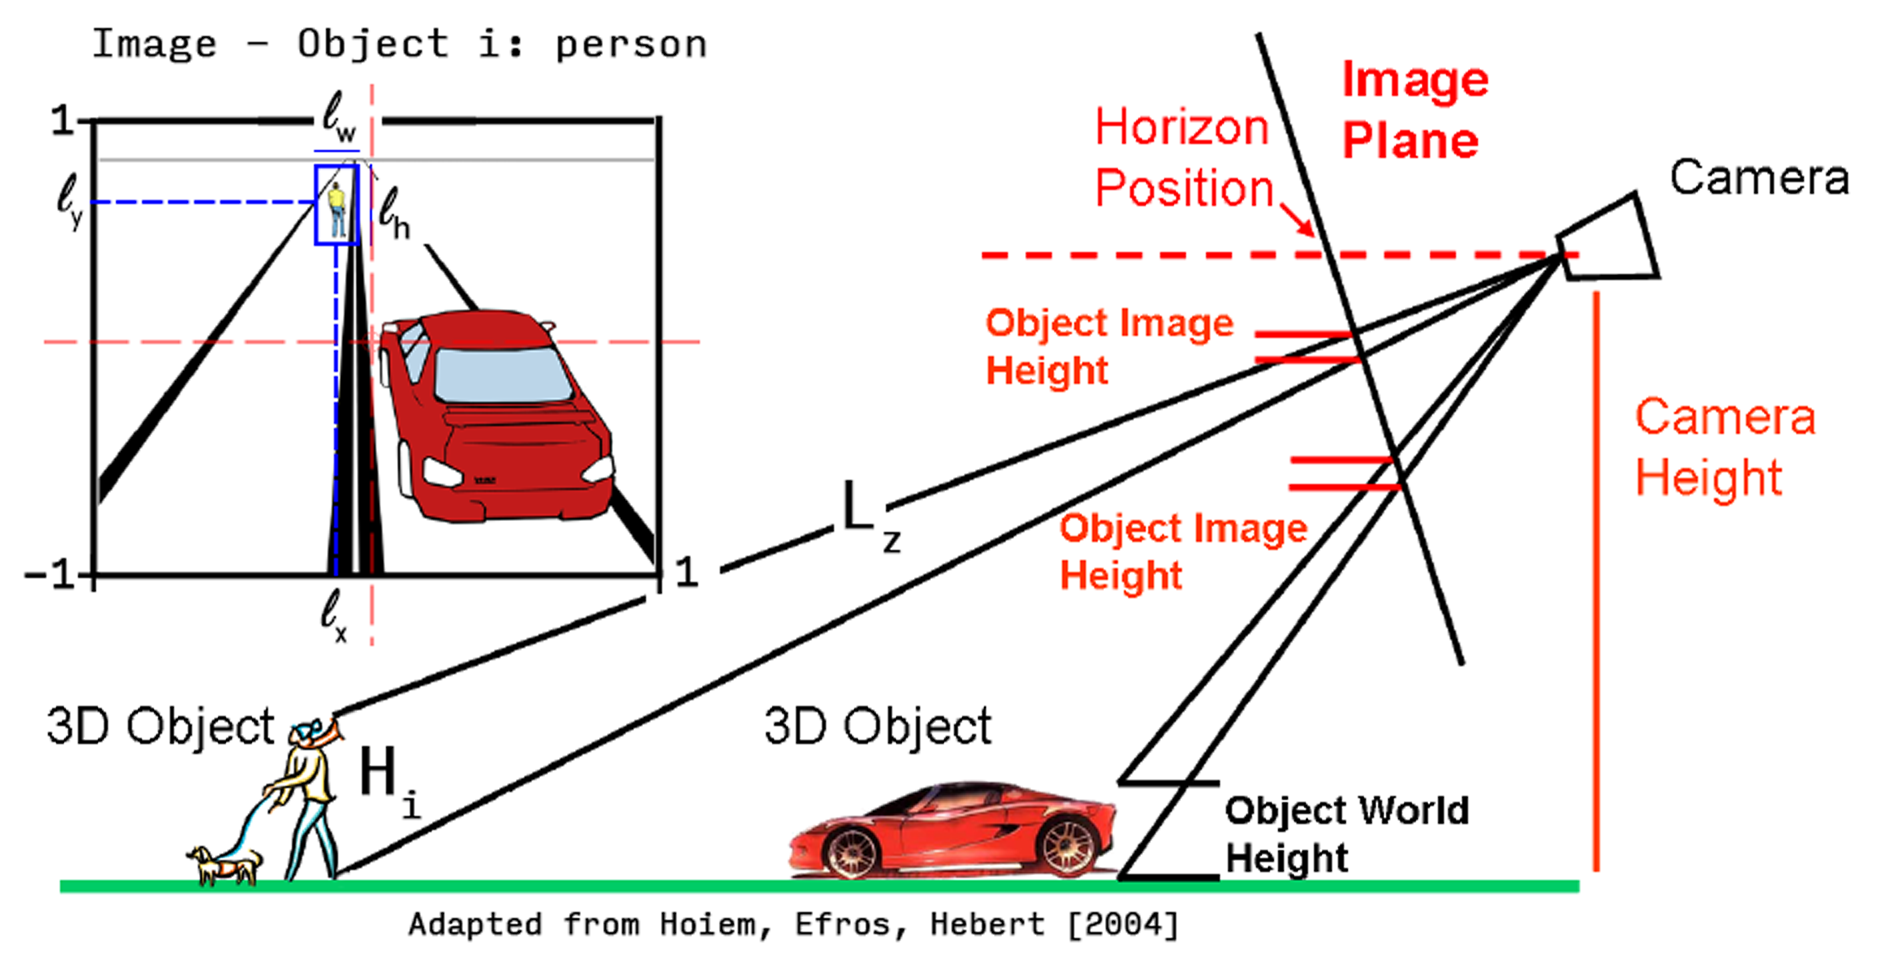
\includegraphics[width=12cm]{3DC.png}
	\end{figure}
	\begin{itemize}
	\item Horizontal locations dropped since they tend to have weak contextual information!
	\item We assume $(L_y^{(i)})_i$, $(\log L_z^{(i)})_i$ are jointly Gaussians and that $L|b$ inherits the binary prior tree structure. 
	\[\p(L|b)=\p(L_{root}|b_{root})\prod_i\p(L_i|L_{\pi_i},b_i,b_{\pi_i})\tag{Spatial prior}\] 
	\end{itemize}
	
}

\headerbox{The Measurement Model}{name=measur,column=0,below=context}{
	\textcolor{red}{(IV) Baseline detectors}

	We apply \textbf{baseline single-object detectors} to obtain a set of candidate windows (as in $L_i$) for each object category.
	\begin{center}
	\begin{minipage}[c]{.52\linewidth}
    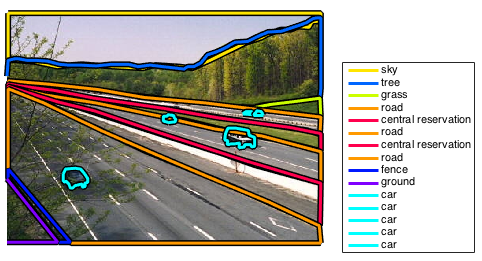
\includegraphics[width=7cm]{local}
	\end{minipage}
	\begin{minipage}[c]{.4\linewidth}
	\begin{itemize}
	\item Candidates : $(W_{i,k})_k$
	\item scores : $(s_{i,k})_k$
	\item verdicts : $(c_{i,k})_k=\mathbb I(\text{correct})$
	\end{itemize}
	\end{minipage}
	\end{center}
	We assume:
	\[W_{i,k}|c_{i,k}=1\sim \gauss(L_i)\:\:W_{i,k}|c_{i,k}=0\sim \mathcal U\indep L_i\]
	\textcolor{red}{(III) GIST}

	We also integrate \textbf{global features} encoded in \texttt{Gist} for each image:
	\begin{enumerate}[label=(\roman*)]
		\item Convolve with 32 \textbf{Gabor filters} at 4 scales, 8 orientations.
		\item Average pooling in a 4x4 grid
		\item Concatenate output: 16x32 descriptor $\equiv$ g.
	\end{enumerate}
	\begin{figure}[H]
    \centering
    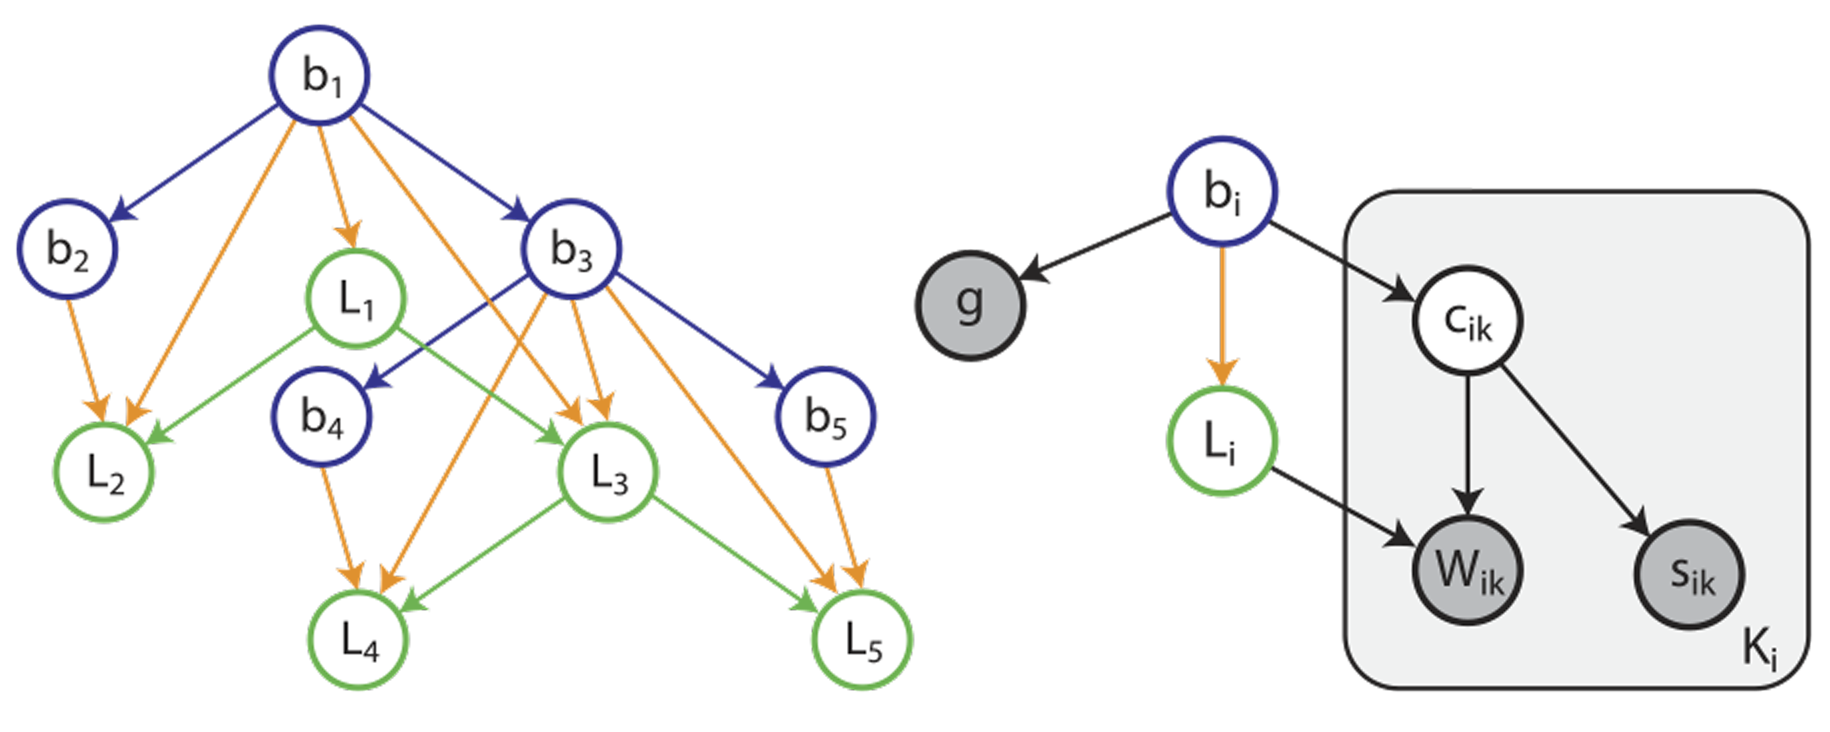
\includegraphics[width=10cm]{tree.png}
	\end{figure}
}



\headerbox{Learning}{name=learn,column=1,row=0}{
\textcolor{red}{(II) The Spatial prior}

Infere $\p(L_i|L_{\pi_i},b_i,b_{\pi_i})$ in 3 scenarios:
\begin{description}
\item[$\mathbf{b_i=1,b_{\pi_i}=1}$] $L_i|L_{\pi_i}\sim\gauss$
\item[$\mathbf{b_i=1,b_{\pi_i}=0}$] $L_i\indep L_{\pi_i}$
\item[$\mathbf{b_i=0}$] $L_i\indep L_j\:\forall j,\text{ set }L_i=\mathbb E(L_i)$
\end{description}

\textcolor{red}{(III) GIST}

For each category fit $\p(b_i|g)$ with a logistic regression.

\textcolor{red}{(IV) Baseline detectors}

For the local detectors outputs, we fit $\p(c_{i,k}|s_{i,k})$ with a logistic regression.

And estimate $\p(c_{i,k} | b_i)$ by counting the correct detections in the training set.
}

\headerbox{Alternating inference on trees - Sum-Product}{name=alt,column=1,below=learn}{
	Inputs: GIST g, candidate windows $W={W_{i,k}}$ and their scores $s={s_{i,k}}$\\
	Infer: Presence $b={b_i}$, detections' verdicts $c={c_{i,k}}$ and the locations $L={L_i}$ as:
	\[\hat b,\hat c,\hat L=\arg\max_{b,c,L} \p(b,c,L|g,s,W)\]
	Noting that $L|b,c$ is a Gaussian tree and $b,c|L$ is a Binary tree

	\textcolor{blue}{Approach:}\\
	\textcolor{blue}{Initialisation:}
	\[\hat b,\hat c=\arg\max_{b,c}\p(b,c|g,s)\tag{Ignoring W}\]
	\textcolor{blue}{Iterate:}
	\[\hat L=\arg\max_L\p(L|\hat b,\hat c,W)\tag{Gaussian tree : SUM-PRODUCT}\]
	\[\hat b,\hat c=\arg\max_{b,c}\p(b,c|g,s)\p(\hat L,W|b,c)\tag{Binary tree: SUM-PRODUCT}\]
	\textcolor{blue}{Final outputs:}\\
	Compute marginal probability $\p(b_i=1|g,s,\hat L,W)$\\
	And the marginal $\p(c_{i,k}=1|g,s,\hat L,W)$

	To deal with re-occurring objects of class $i$, we set all the messages from node $b_i$ to $(c_{i,k})_{1\leq k\leq K_i}$ as 1, except a single occurence.
}

\headerbox{Experiments - SUN 09}{name=sun,column=1,below=alt}{
\textbf{Dataset: SUN 09, Training: 4367 images, Test: 4317, N=111 categories.}\\
\textcolor{plum}{\bf Object dependency structure learned from SUN 09 - subtree \texttt{Floor}:}
\begin{figure}[H]
    \centering
    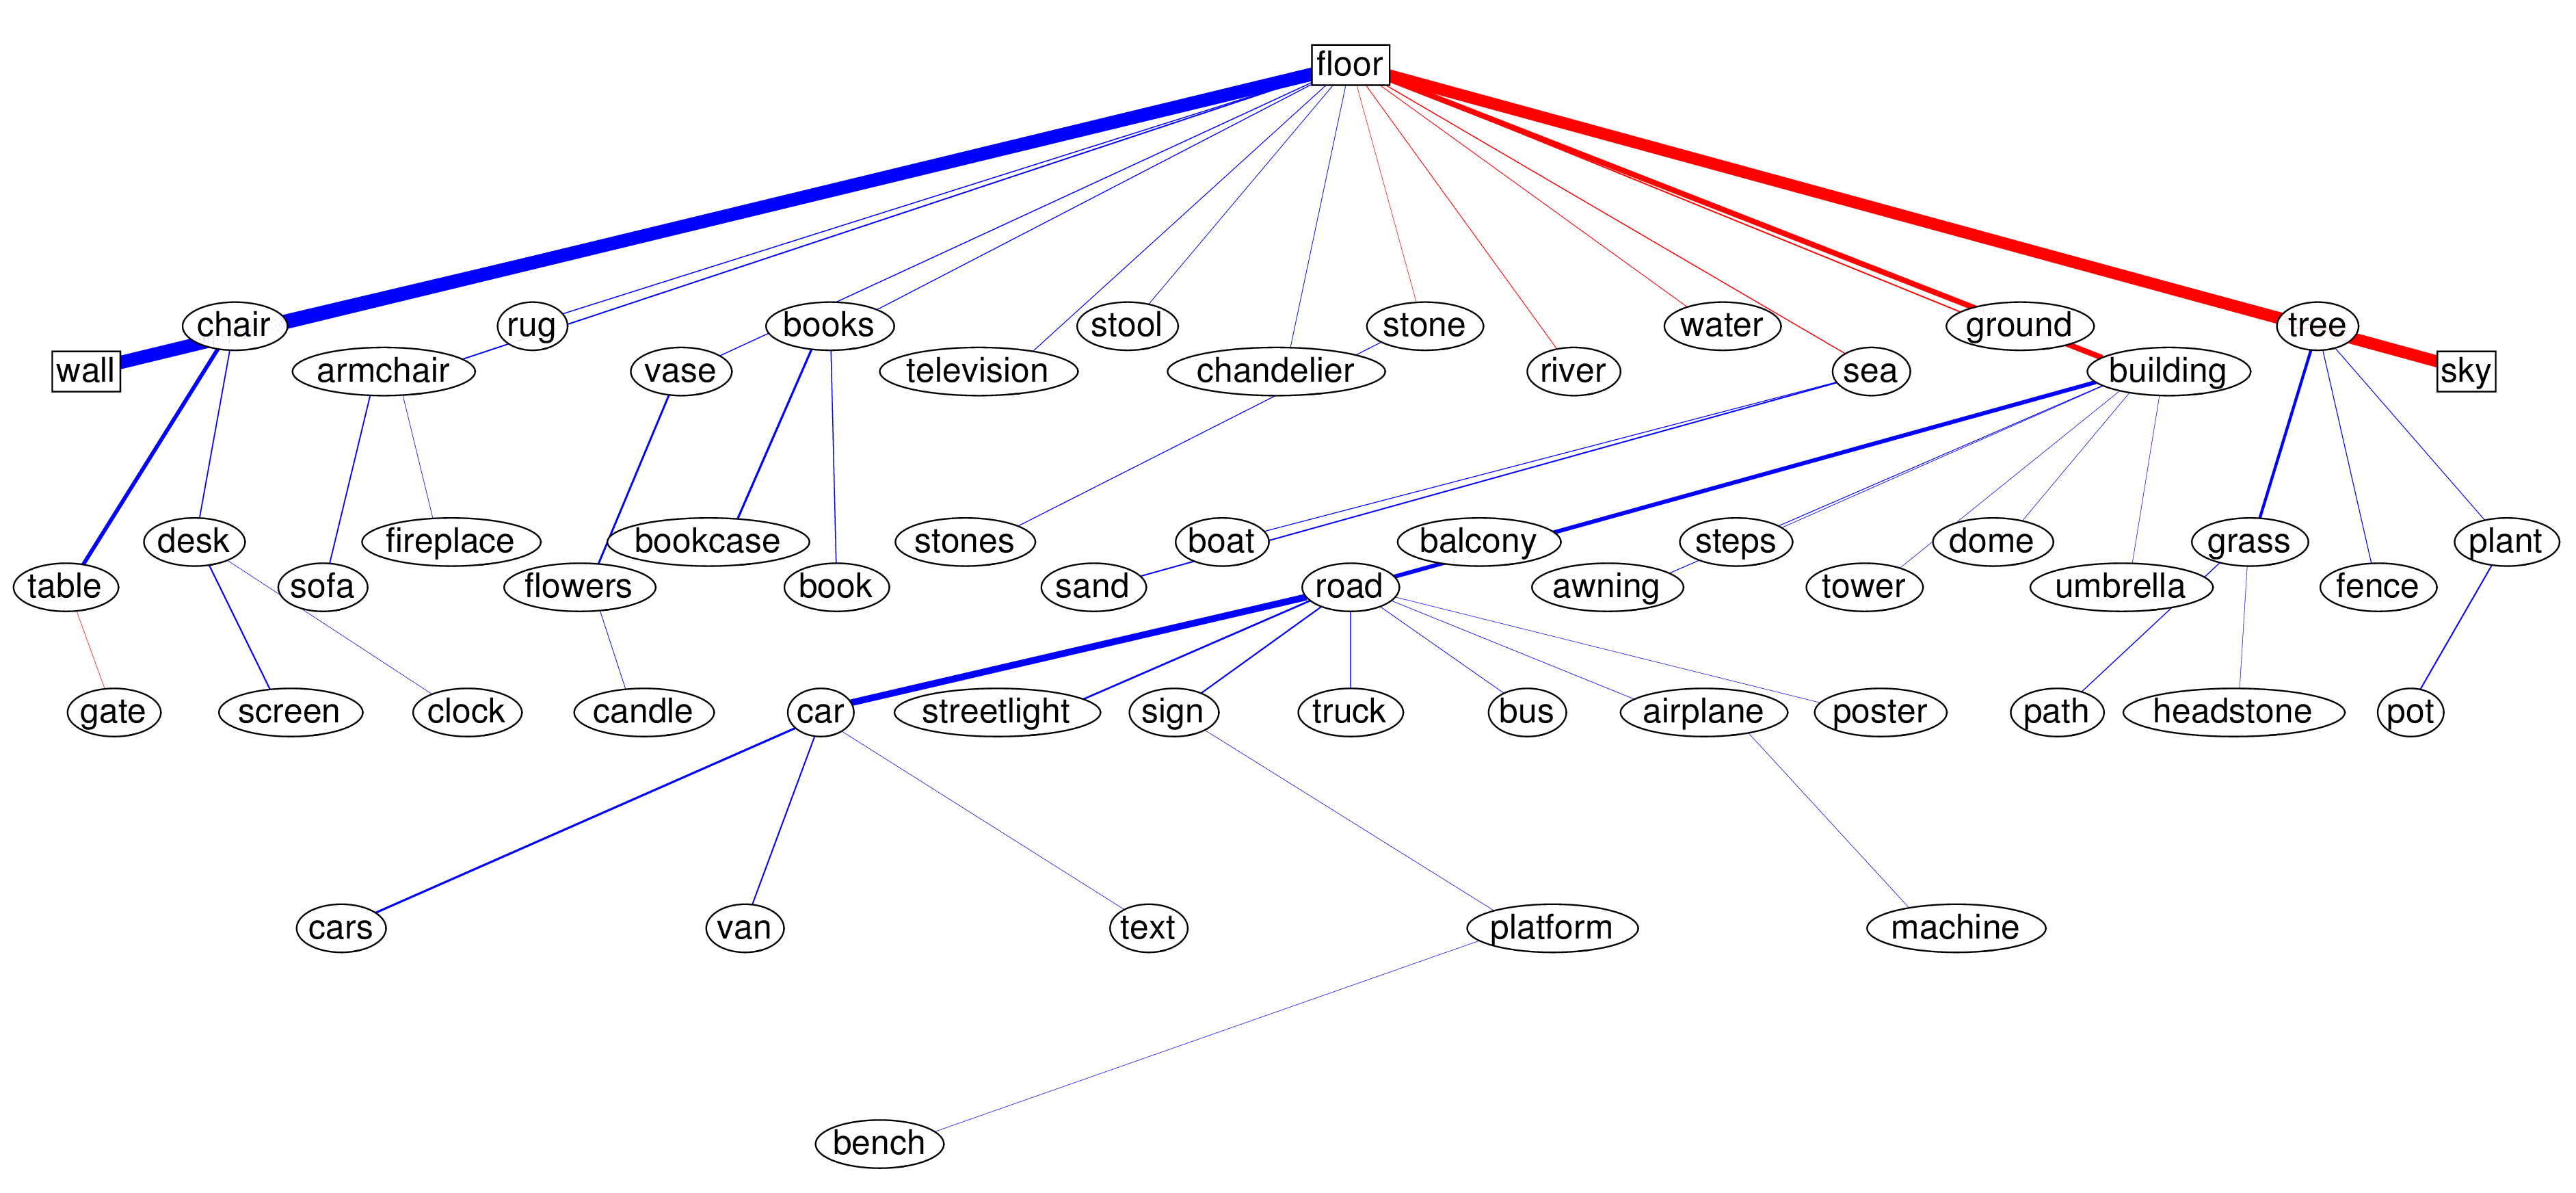
\includegraphics[width=12cm]{floor.png}
\end{figure}
\textcolor{plum}{\bf Localisation and presence prediction performance:}
\begin{center}
\begin{minipage}[c]{.48\linewidth}
    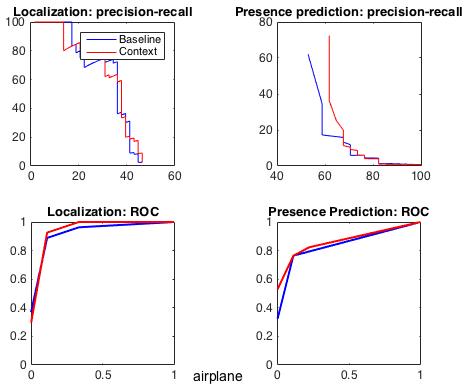
\includegraphics[width=6cm]{airplane}
\end{minipage}
\begin{minipage}[c]{.48\linewidth}
    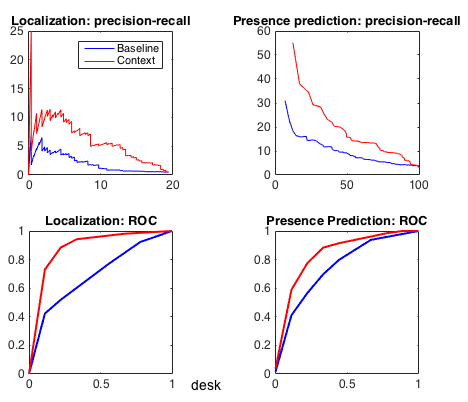
\includegraphics[width=6cm]{desk}
\end{minipage}
\end{center}

\textcolor{plum}{\bf Average recognition performance for the top N most confident detections}
\begin{figure}[H]
    \centering
    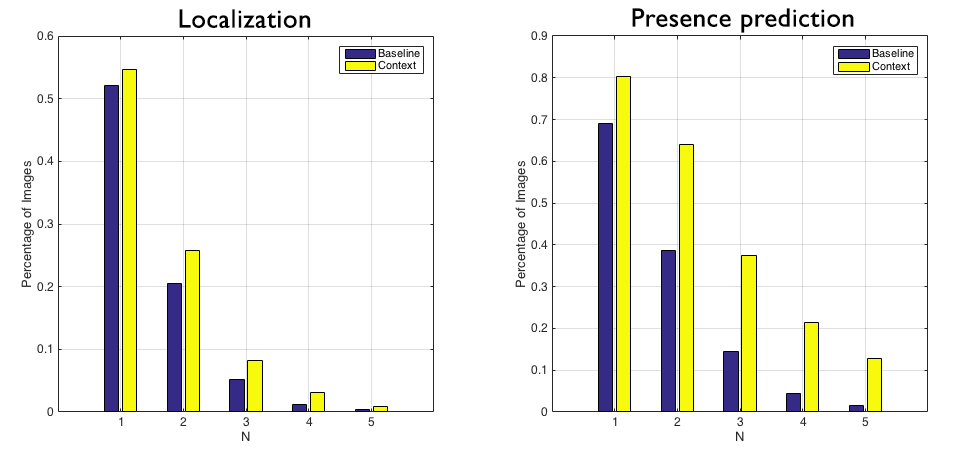
\includegraphics[width=10cm]{perf}
\end{figure}
}

\end{poster}

\end{document}